\appendix 

\Chapter{Railroad diagramok}
\label{sec:rr_melleklet}

A melléklet a grammatika főbb szabályainak railroad diagramjait tartalmazza, a legáltalánosabb szabálytól a specifikusabbak felé haladva.

\begin{figure}[H]
	\centering
	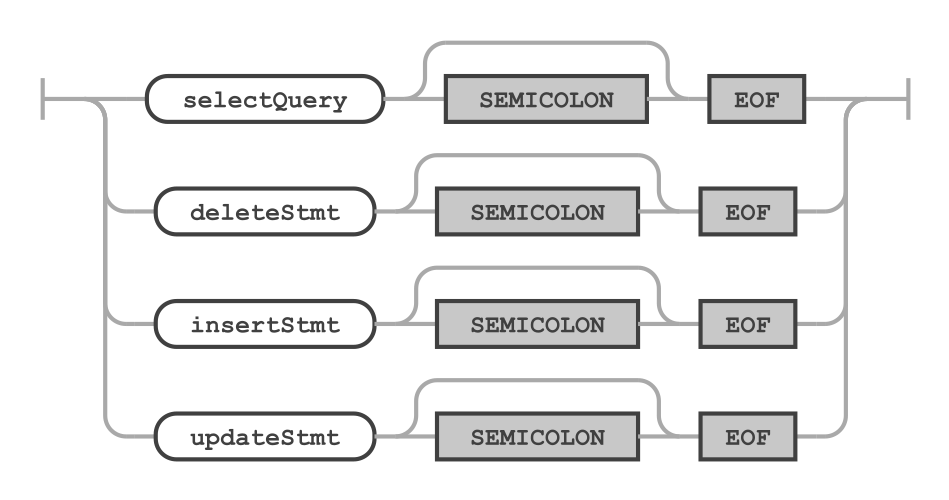
\includegraphics[width=0.9\textwidth]{figures/query.png}
	\caption{A \texttt{query} szabály railroad diagramja}
	\label{fig:rr_query}
\end{figure}

\begin{figure}[H]
	\centering
	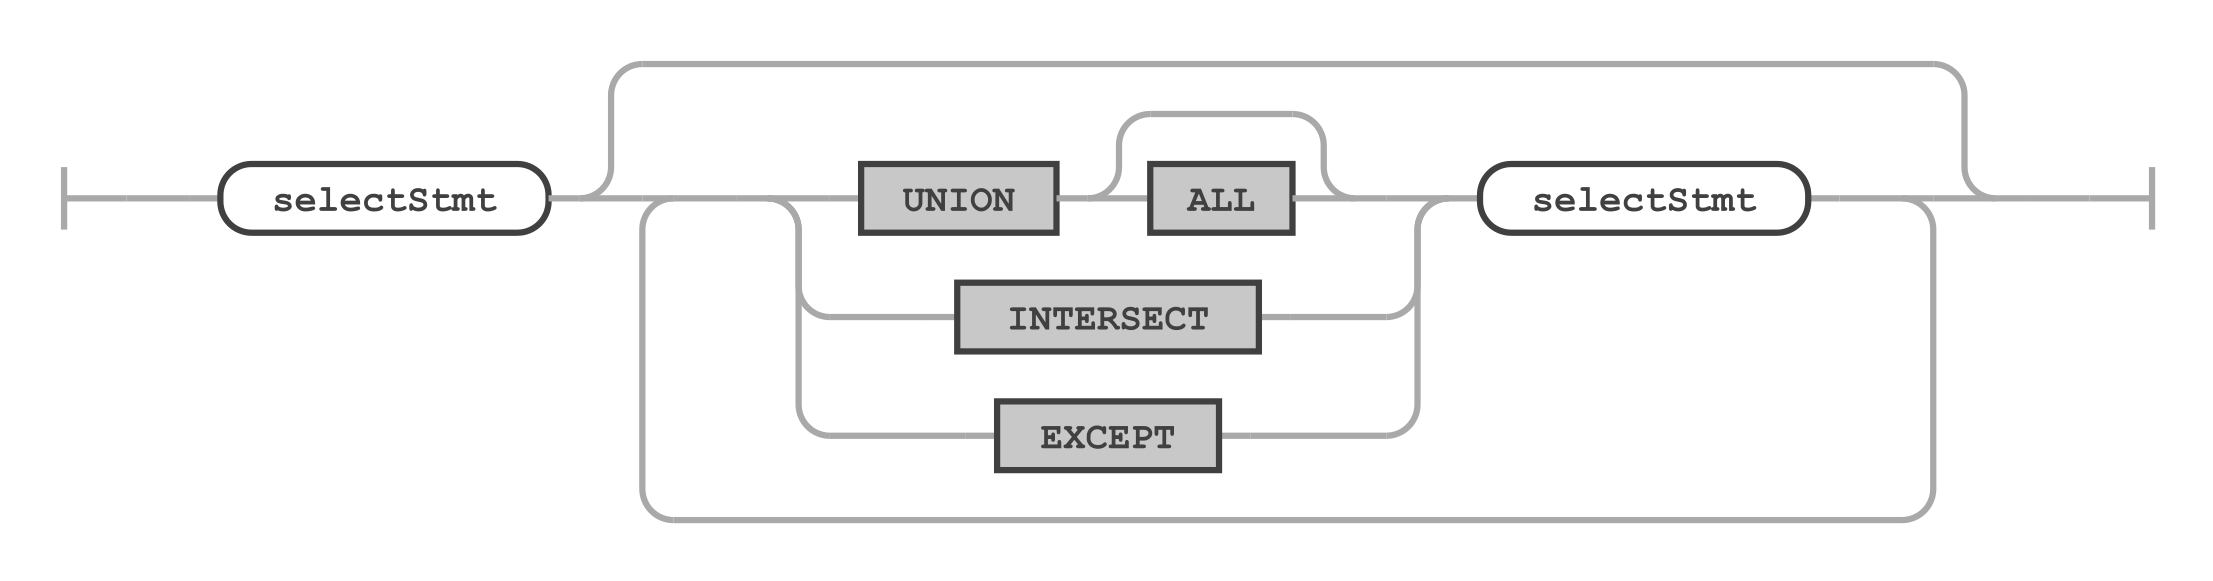
\includegraphics[width=\textwidth]{figures/selectQuery.png}
	\caption{A \texttt{selectQuery} szabály railroad diagramja}
	\label{fig:rr_selectquery}
\end{figure}

\begin{figure}[H]
	\centering
	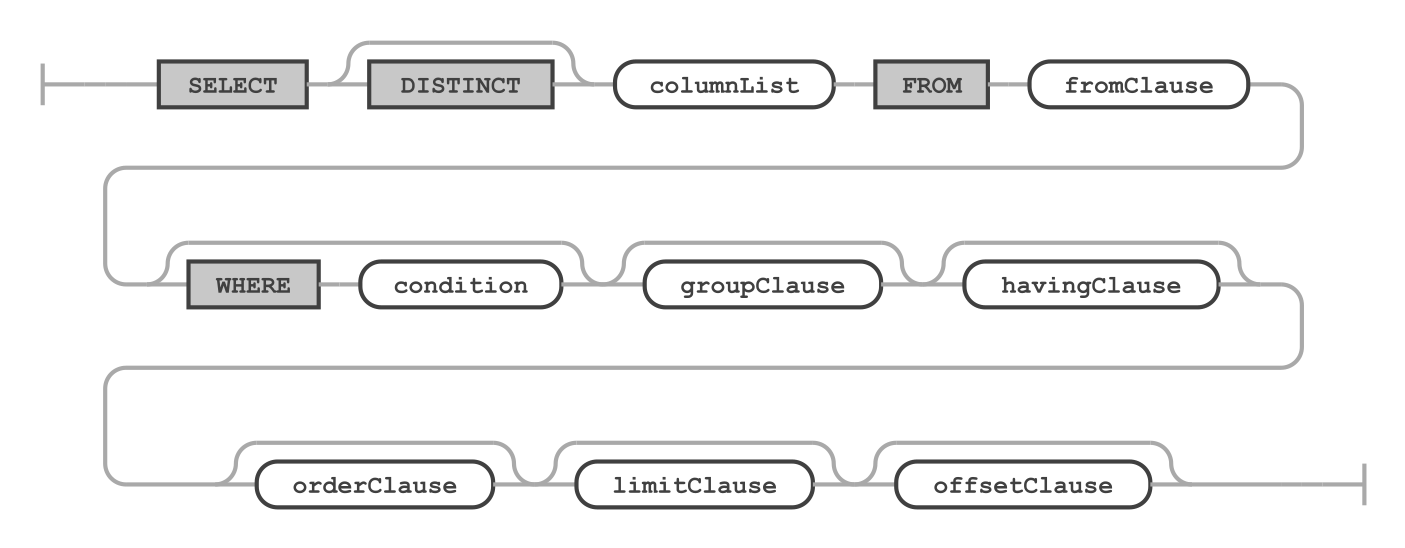
\includegraphics[width=\textwidth]{figures/selectStmt.png}
	\caption{A \texttt{selectStmt} grammatikai szabály railroad diagramja}
	\label{fig:rr_selectstmt}
\end{figure}

\begin{figure}[H]
	\centering
	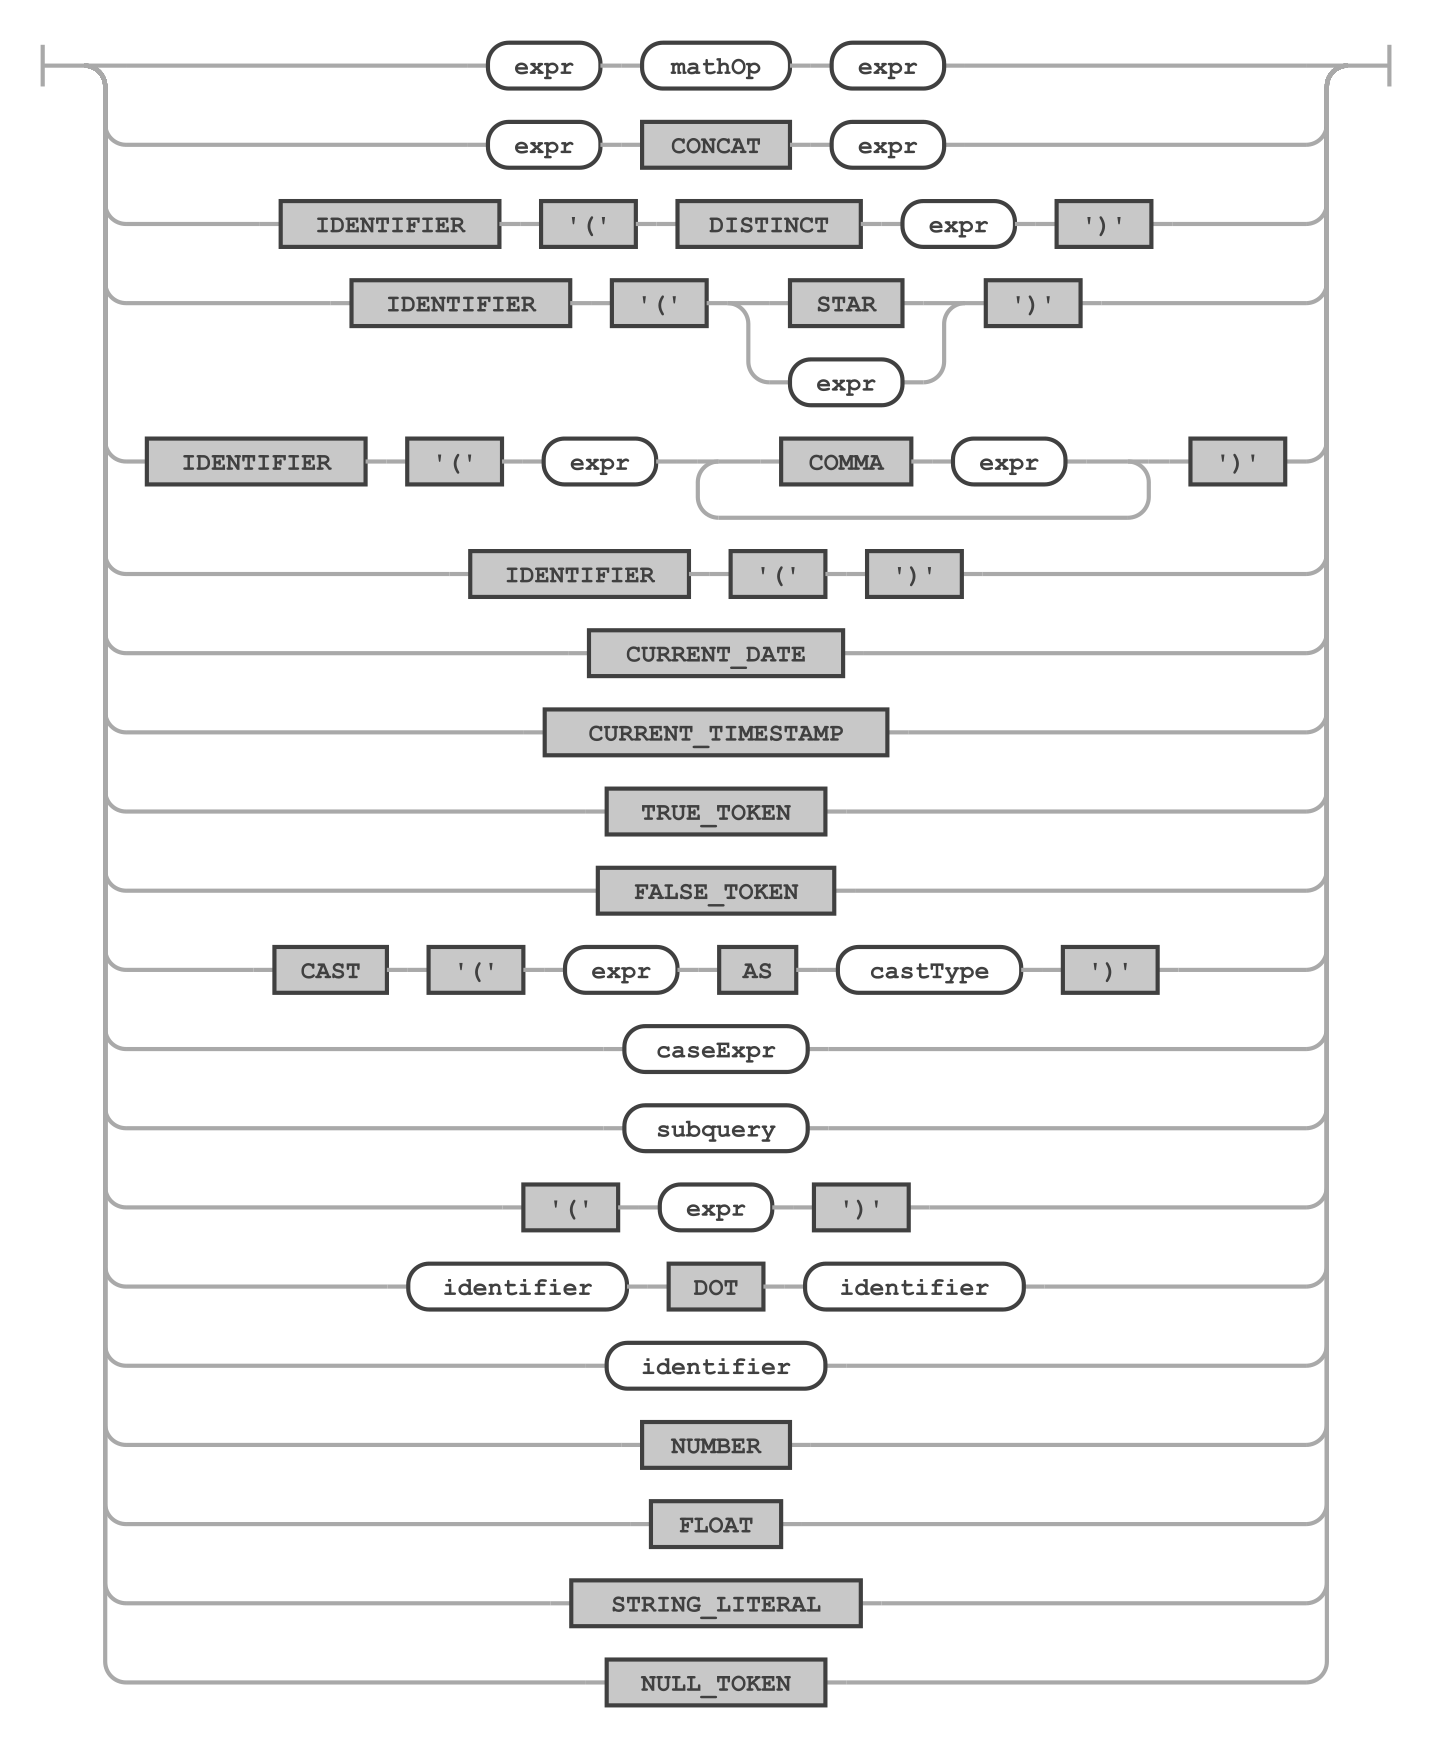
\includegraphics[width=\textwidth]{figures/expr.png}
	\caption{Az \texttt{expr} grammatikai szabály railroad diagramja}
	\label{fig:rr_expr}
\end{figure}

\begin{figure}[H]
	\centering
	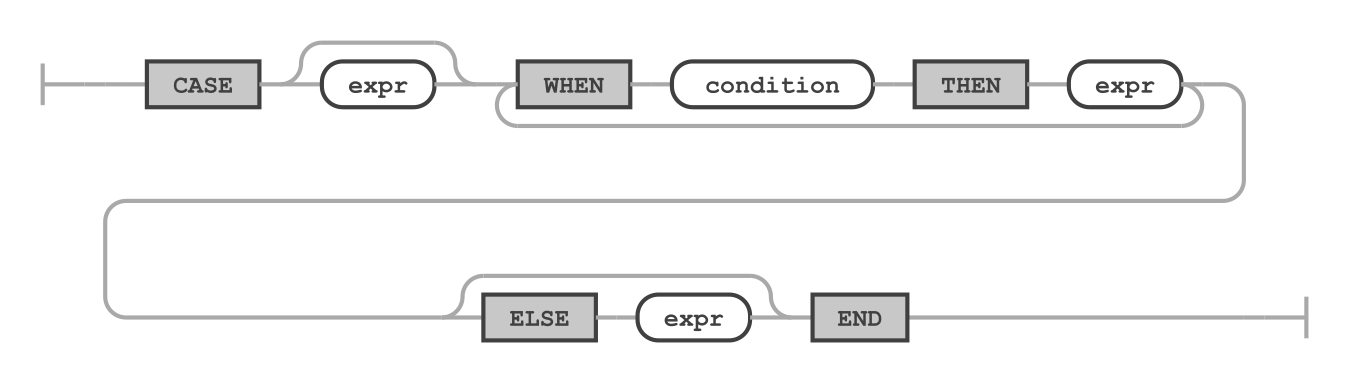
\includegraphics[width=\textwidth]{figures/caseExpr.png}
	\caption{A \texttt{caseExpr} grammatikai szabály railroad diagramja}
	\label{fig:rr_caseexpr}
\end{figure}

\Chapter{Az LLM-mérés lekérdezései}
\label{sec:llm_melleklet}

A mérésben minden modell ugyanazt a promptot kapta, amelyben a \texttt{\{sql\}} helyére az adott lekérdezés szövege került. Az utasítás a promptban egyetlen sor, az itt látható sortörések csak a tördelés miatt szerepelnek.

\begin{lstlisting}[language={}, caption={A modelleknek küldött prompt sablonja}, label={lst:llm_prompt}]
	Convert the following SQL query to C# LINQ method
	syntax compatible with Entity Framework Core 8.
	Respond with the LINQ expression only, without any
	explanation or markdown formatting.
	
	SQL:
	{sql}
\end{lstlisting}

A mért lekérdezéseket az alábbi kódpéldák tartalmazzák. A modellek a lekérdezéseket egyetlen sorban kapták meg, az itt látható tördelés csak az olvashatóságot szolgálja.

\begin{lstlisting}[language=SQL, caption={Q1, egyszerű szűrés és rendezés}, label={lst:llm_q1}]
	SELECT Name, Age
	FROM Users
	WHERE Age > 18
	ORDER BY Name ASC
\end{lstlisting}

\newpage

\begin{lstlisting}[language=SQL, deletekeywords={ROLE}, caption={Q2, csoportosítás, HAVING feltétel és rendezés az aggregátum aliasára}, label={lst:llm_q2}]
	SELECT Role, COUNT(*) AS Cnt
	FROM Users
	WHERE Age >= 18
	GROUP BY Role
	HAVING COUNT(*) > 1
	ORDER BY Cnt DESC
\end{lstlisting}

\begin{lstlisting}[language=SQL, caption={Q3, kéttáblás LEFT JOIN szűréssel, rendezéssel és lapozással}, label={lst:llm_q3}]
	SELECT u.Name, o.Item
	FROM Users u
	LEFT JOIN Orders o ON u.Id = o.Owner
	WHERE u.Age >= 25
	ORDER BY u.Name DESC
	LIMIT 4
\end{lstlisting}

\begin{lstlisting}[language=SQL, caption={Q4, CASE WHEN kifejezés és korrelált EXISTS allekérdezés}, label={lst:llm_q4}]
	SELECT Name,
	CASE WHEN Age > 40 THEN 'Senior'
	WHEN Age > 25 THEN 'Mid'
	ELSE 'Junior'
	END AS Level
	FROM Users u
	WHERE EXISTS (SELECT 1 FROM Orders o WHERE o.Owner = u.Id)
	ORDER BY Name ASC
\end{lstlisting}

\begin{lstlisting}[language=SQL, caption={Q5, háromtáblás JOIN összetett feltétellel, LIKE mintával, LIMIT és OFFSET záradékkal}, label={lst:llm_q5}]
	SELECT u.Name, o.Item, p.Title
	FROM Users u
	JOIN Orders o ON u.Id = o.Owner
	JOIN Products p ON o.Id = p.Parent
	WHERE u.Name LIKE 'B%' AND (o.Qty >= 1 OR p.Price < 20)
	ORDER BY p.Price DESC
	LIMIT 5 OFFSET 1
\end{lstlisting}
